\documentclass[tikz,border=8pt]{standalone}
\usepackage{pgfplots}
\pgfplotsset{compat=1.18}
\definecolor{ink}{HTML}{17324D}
\definecolor{teal}{HTML}{168C80}
\definecolor{gold}{HTML}{D79A2B}
\definecolor{rose}{HTML}{C85B70}
\begin{document}
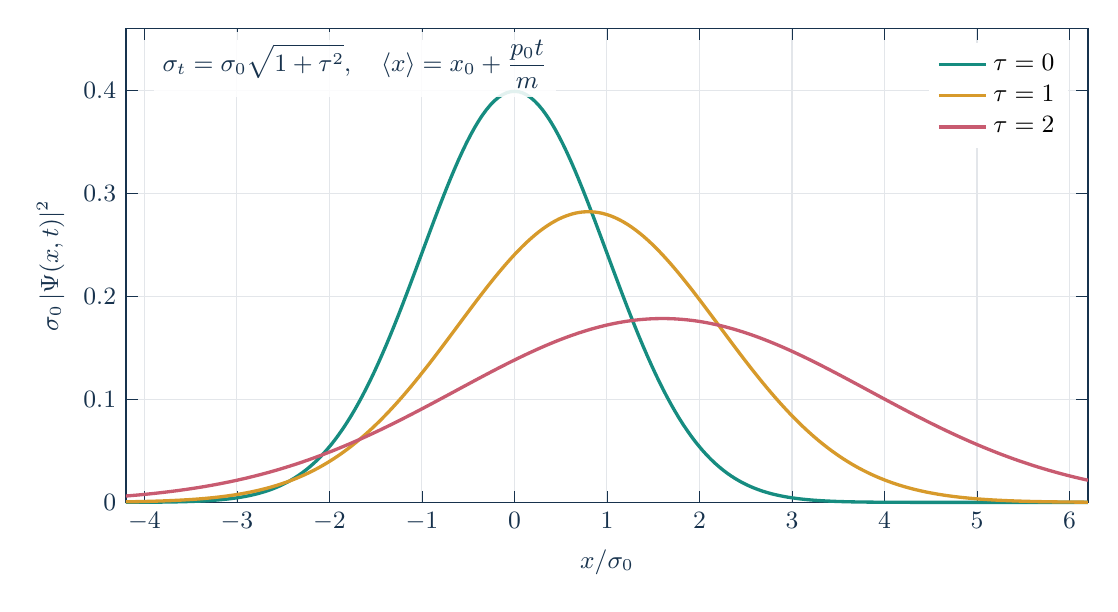
\begin{tikzpicture}
  \begin{axis}[
    width=13.8cm,
    height=7.6cm,
    xmin=-4.2,xmax=6.2,
    ymin=0,ymax=0.46,
    axis line style={ink,semithick},
    tick style={ink},
    tick label style={font=\small,text=ink},
    label style={font=\small,text=ink},
    xlabel={$x/\sigma_0$},
    ylabel={$\sigma_0\,|\Psi(x,t)|^2$},
    grid=major,
    grid style={draw=ink!12},
    legend style={draw=none,fill=white,font=\small,at={(0.98,0.97)},anchor=north east},
    samples=241,
    domain=-4.2:6.2,
    clip=false
  ]
    % Dimensionless form: sigma_t/sigma_0=sqrt(1+tau^2), centre=0.8 tau.
    \addplot[very thick,teal]
      {1/sqrt(2*pi)*exp(-x^2/2)};
    \addlegendentry{$\tau=0$}
    \addplot[very thick,gold]
      {1/(sqrt(2*pi)*sqrt(2))*exp(-(x-0.8)^2/(2*2))};
    \addlegendentry{$\tau=1$}
    \addplot[very thick,rose]
      {1/(sqrt(2*pi)*sqrt(5))*exp(-(x-1.6)^2/(2*5))};
    \addlegendentry{$\tau=2$}
    \node[anchor=west,font=\small,text=ink,fill=white,fill opacity=.88,text opacity=1,inner sep=3pt]
      at (axis cs:-3.9,0.425)
      {$\displaystyle \sigma_t=\sigma_0\sqrt{1+\tau^2},\quad
        \langle x\rangle=x_0+\frac{p_0t}{m}$};
  \end{axis}
\end{tikzpicture}
\end{document}
